\documentclass[extra,mreferee]{gji}
%\documentclass[extra,onecolumn,doublespacing]{gji}
\usepackage{timet}
\usepackage{amsmath}
\usepackage{amsfonts}
\usepackage{amssymb}
\usepackage{graphicx}
\usepackage{arydshln}
\usepackage{bm}
\usepackage{ulem}

\title[Transient strain in geodetic data]
      {Revealing transient strain in geodetic data with Gaussian process regression}

\author[T. T. Hines and E. A. Hetland]
       {T. T. Hines$^1$ and E. A. Hetland$^1$ \\
        $^1$ Department of Earth and Environmental Sciences, University of Michigan, Ann Arbor, MI, USA}

\date{Received XXX; in original form XXX}

\pagerange{\pageref{firstpage}--\pageref{lastpage}}

\volume{XXX}

\pubyear{XXX}

% Authors with AMS fonts and mssymb.tex can comment out the following
% line to get the correct symbol for Geophysical Journal International.
\let\leqslant=\leq

\newtheorem{theorem}{Theorem}[section]

\begin{document}

\label{firstpage}

\maketitle

%% DEFINE MATH MODE MACROS
%%%%%%%%%%%%%%%%%%%%%%%%%%%%%%%%%%%%%%%%%%%%%%%%%%%%%%%%%%%%%%%%%%%%%
\newcommand{\pos}{\vec{x}} % position vector
\newcommand{\data}{\mitbf{d}} % data vector
\newcommand{\post}{\hat{u}} % posterior
\newcommand{\points}{\mitbf{P}} % observation points
\newcommand{\strain}{\dot\varepsilon} % strain rate
\newcommand{\E}[1]{\mathrm{E}\left[ #1 \right]} % Expected value
\newcommand{\Cov}[1]{\mathrm{Cov}\left[ #1 \right]} % Expected value
\newcommand{\e}{\mathrm{e}} % east subscript
\newcommand{\n}{\mathrm{n}} % north subscript
\newcommand{\G}{\mitbf{G}} % basis functions
\newcommand{\zeros}{\mitbf{0}} % zeros matrix
\newcommand{\eye}{\mitbf{I}} % identity matrix

%% SUMMARY
%%%%%%%%%%%%%%%%%%%%%%%%%%%%%%%%%%%%%%%%%%%%%%%%%%%%%%%%%%%%%%%%%%%%%
\begin{summary}

% focus on subjective vs object rather than "we have uncertainties"

Transient strain rates derived from GNSS data can be used to detect
and understand geophysical processes such as slow slip events and
postseismic deformation. Here we propose using Gaussian process
regression (GPR) as a tool for estimating transient strain rates from
GNSS data. GPR is a non-parametric, Bayesian method for interpolating
scattered data. In our approach, we assume a stochastic prior model
for transient displacements. The prior describes how much we expect
transient displacements to covary spatially and temporally. A
posterior estimate of transient strain rates is obtained by
differentiating the posterior displacements. As a demonstration, we
use GPR to detect transient strain resulting from slow slip events in
the Pacific Northwest. Maximum likelihood methods are used to
constrain a prior model for transient displacements in this region.
The temporal covariance of our prior model is described by a compact
Wendland covariance function, which significantly reduces the
computational burden that can be associated with GPR. Our results
reveal the spatial and temporal evolution of strain from slow slip
events. We verify that the transient strain estimated with GPR is in
fact geophysical signal by comparing it to the seismic tremor that is
associated with Pacific Northwest slow slip events.

\end{summary}

\begin{keywords}
 XXX -- XXX -- XXX -- XXX.
\end{keywords}

%% INTRODUCTION
%%%%%%%%%%%%%%%%%%%%%%%%%%%%%%%%%%%%%%%%%%%%%%%%%%%%%%%%%%%%%%%%%%%%%
\section{Introduction}\label{sec:Introduction}

% Why we care about determining strain

Crustal strain rates are fundamentally important quantities for
assessing seismic hazard. Knowing where and how quickly strain is
accumulating gives insight into where we can expect stored elastic
energy to be released seismically. Consequently, secular crustal
strain rates estimated from GNSS data have been used to constrain
seismic hazard models such as UCERF3 \citep{Field2014}. Transient
crustal strain, which is caused by geophysical phenomena such as slow
slip events (SSEs) or postseismic deformation, is also relevant for
assessing seismic hazard. While transient strain itself is not
damaging, there is a risk that it can trigger major earthquakes
\citep{Roeloffs2006,Freed2001}. Dense networks of continuous GNSS
stations, such as the Plate Boundary Observatory (PBO), make it
possible to identify transient strain with high fidelity. Developing
and improving upon methods for deriving secular and transient strain
from GNSS data is an active area of research.

% Existing methods for determining secular strain from GPS

Most methods for estimating strain rates from GNSS data assume some
parametric form for the deformation signal. The simplest method for
estimating secular strain rates assumes that GNSS derived velocities
can be described with a first-order polynomial (i.e, the deformation
gradients are constant) over some subnetwork of the GNSS stations
\citep[e.g.,][]{Feigl1990,Murray2000}. The components of the strain
rate tensor for each subnetwork are then determined from the least
squares fit to the observations. The assumption that deformation
gradients are spatially uniform is not appropriate when subnetworks
span too large of an area. To help overcome this deficiency,
\citet{Shen1996,Shen2015} used an inverse distance weighting scheme,
in which the estimated strain rate at a point is primarily controlled
by observations at nearby stations. The method of
\citet{Shen1996,Shen2015} can be viewed as a form of local least
squares regression with a first-order polynomial \citep[e.g.,][sec.
6]{Hastie2009}. Other methods for estimating secular strain rates have
parameterized GNSS derived velocities with bi-cubic splines
\citep{Beavan2001}, spherical wavelets \citep{Tape2009}, and
elastostatic Green's functions \citep{Sandwell2016}. The type of basis
functions and the number of degrees of freedom for a parameterization,
which are often chosen subjectively, have a strong influence on the
strain solution. If there are too few degrees of freedom in the
parameterization, then estimated strain rates will be biased and the
uncertainties will be underestimated. On the other hand, if there are
too many degrees of freedom, then there will not be any coherent
features in the estimated strain rates. The methods described by
\citet{Beavan2001} and \citet{Tape2009} also require the user to
specify penalty parameters that control a similar trade-off between
bias and variance in the solution. One could parameterize deformation
with a physically motivated model of interseismic deformation
\citep[e.g.,][]{Meade2005,McCaffrey2007}. In such models the
lithospheric rheology and fault geometries are assumed to be known.
Any errors in the assumed physical model could result in biased strain
estimates and underestimated formal uncertainties.

% Existing methods for determining transient strain from GPS

The aforementioned studies are concerned with estimating secular
strain rates. In recent years the Southern California Earthquake
Center (SCEC) community has shown interest in developing methods for
detecting transient strain. SCEC supported a transient detection
exercise \citep{Lohman2013}, where several research groups tested
their methods for detecting transient geophysical signal with a
synthetic GNSS dataset. Among the methods tested were the Network
Strain Filter (NSF) \citep{Ohtani2010} and the Network Inversion
Filter (NIF) \citep{Segall1997}. The NSF uses a wavelet
parameterization to describe the spatial component of geophysical
signal. The NIF, which is intended for imaging slow fault slip from
geodetic data, uses the elastic dislocation Green's functions from
\citet{Okada1992}. For the NSF and NIF, the time dependence of the
geophysical signal is modeled as integrated Brownian motion. The
method described in \citet{Holt2013} was also tested in the SCEC
transient detection exercise, which calculates strain rates using a
bi-cubic spatial parameterization of displacements between time
epochs. \citet{Holt2013} defined a detection threshold based on the
strain rate magnitude, and we demonstrate that this is indeed an
effective criterion for identifying geophysical signal. For the same
reasons descibed above, the transient deformation and corresponding
uncertainties estimated by these methods can be biased by the chosen
spatial parameterization. It is then difficult to distinguish signal
from noise with these methods, which limits their utility for
transient detection.

% What we are doing in this paper and why it improves upon existing
% methods

Here we propose using Gaussian process regression (GPR)
\citep{Rasmussen2006} to estimate transient strain from GNSS data. GPR
is closely related to kriging \citep{Cressie1992} and least squares
collocation \citep{Moritz1978}. The latter has been used by
\citet{Kato1998} and \citet{El-Fiky1999} to estimate secular strain
rates from GNSS data. GPR is a Bayesian, non-parametric method for
inferring a continuous signal from scattered data. Since GNSS stations
are irregularly spaced and observation times may differ between
stations, GPR is an ideal tool for synthesizing discrete GNSS data
into a spatially and temporally continuous representation of transient
strain. GPR is Bayesian in that we use a prior model to control the
spatial and temporal roughness of the inferred transient strain. The
prior is specified as a stochastic process, namely a Gaussian process.
If there is no information available to help choose an appropriate
prior Gaussian process, then maximum likelihood methods can be used to
objectively choose one that is most consistent with the data. We use
GPR to infer transient strain resulting from SSEs in the Pacific
Northwest, demonstrating that GPR is an effective tool for detecting
transient geophysical processes.


%% ESTIMATING TRANSIENT STRAIN RATES
%%%%%%%%%%%%%%%%%%%%%%%%%%%%%%%%%%%%%%%%%%%%%%%%%%%%%%%%%%%%%%%%%%%%%
\section{Estimating Transient Strain Rates}\label{sec:Method}

% Overview of what we are trying to do in this section and how

We seek a spatially and temporally dependent estimate of transient
strain rates. We consider transient strain rates to be any deviation
from the secular strain rates. We denote transient strain rates as
$\strain(p)$, where $p$ represents the ordered pair $(\pos,t)$, $\pos
= (x_\e,x_\n)$ are spatial coordinates, and $t$ is time. The
subscripts ``e" and ``n" indicate the east and north component, and we
assume that the study region is sufficiently small that $\pos$ can be
considered a point in a 2-D Cartesian map projection that is aligned
with the cardinal directions. We determine $\strain$ by spatially and
temporally differentiating estimates of transient displacements, which
we constrain with GNSS data.

% Defining u as a prior Gaussian process

We let $\vec{u}(p) = (u_\e(p),u_\n(p))$ be our prior understanding of
transient displacements. Since transient displacements are not
precisely known, we cannot consider $\vec{u}$ to be a deterministic
function. Instead, $\vec{u}$ is considered to be a stochastic process
containing a distribution of functions that could potentially describe
transient displacements. Specifically, we let each component of
$\vec{u}$ be a Gaussian process. A Gaussian process is a stochastic
process whose value at any collection of points can be described with
a multivariate normal distribution. That is to say, the random vector
$[u_i(p)]_{p \in \points}$ has a multivariate normal distribution for
any collection of points $\points$. A realization of the random vector
$[u_i(p)]_{p \in \points}$ can be interpretted as a realization of
$u_i$ (i.e., a sample function) that is evaluated at $\points$. Just
as a multivariate normal distribution is fully determined by a mean
vector and a covariance matrix, a Gaussian process is fully determined
by a mean function and a covariance function. For example, Brownian
motion, $B(t)$, is a well known Gaussian process in $\mathbb{R}^1$
which has the mean function $\E{B(t)} = 0$ and the covariance function
$\Cov{B(t),B(t')} = \min(t,t')$, where $t,t' \ge 0$. We let each
component of $\vec{u}$ have zero mean and a generic covariance
function $\Cov{u_i(p),u_i(p')} = C_{u_i}(p,p')$. Using a more concise
notation, we write our prior on each component of $\vec{u}$ as $u_i
\sim \mathcal{GP}\left(0,C_{u_i}\right)$.

% Constraints on the Covariance function

The function $C_{u_i}$ must be positive definite in order to be a
valid covariance function. By definition, $C_{u_i}$ is a positive
definite function if the matrix $[C_{u_i}(p,p')]_{(p,p') \in \points
\times \points}$ is positive definite for any set of points $\points$
\citep[sec. 2.5]{Cressie1992}. We assume that $C_{u_i}$ can be
separated into spatial and temporal functions as
\begin{equation}\label{eq:TransientCovariance}
C_{u_i}(p,p') = C_{u_i}\left((\pos,t),(\pos',t')\right) 
              = X_i(\pos,\pos')T_i(t,t').
\end{equation}   
As long as the functions $X_i$ and $T_i$ are positive definite,
$C_{u_i}$ is guaranteed to also be positive definite \citep[sec.
4.2.4]{Rasmussen2006}. We also require that the derivatives
$\partial^2 X_i(\pos,\pos')/ \partial x_j \partial x_j'$ and
$\partial^2 T_i(t,t') / \partial t \partial t'$ exist. This ensures
that $u_i$ is spatially and temporally differentiable, allowing us to
compute transient strain rates (See \citet[sec. 2.2]{Adler1981} or
\citet[sec. 10A]{Papoulis1991} for a definition of stochastic
differentiation and the conditions for differentiability).

% Example of the prior

We provide an example to give the prior on transient displacements a
more tangible meaning. we can use a squared exponential function for
$X_i$ and $T_i$,
\begin{equation}\label{eq:ExampleCov}
X_i(\pos,\pos') = \exp\left(\frac{-||\pos - \pos'||_2^2}{2\ell^2}\right), \ \ \ \ 
T_i(t,t') = \phi^2 \exp\left(\frac{-|t - t'|^2}{2\tau^2}\right),
\end{equation}
which satisfies our requirements for positive definiteness and
differentiability. The parameters $\ell$ and $\tau$ control the
length-scale and time-scale, respectively, of realizations of $u_i$.
The parameter $\phi$, which we have arbitrarily chosen to incorporate
into $T_i$ rather than $X_i$, controls the amplitude of realizations
of $u_i$. Ideally, we want realizations of $u_i$ to have a
length-scale, time-scale, and amplitude that resemble what we expect
for the true transient displacements. In Figure \ref{fig:PriorDemo}A,
we show $C_{u_i}$ using the squared exponential function for $X_i$ and
$T_i$ and the parameters $\ell = 100$ km, $\tau = 10$ days, and $\phi
= 1$ mm. A single realization of $u_i$ corresponsing to that choice of
covariance function is shown in Figure \ref{fig:PriorDemo}B (See
\citet[sec. A3]{Rasmussen2006} for details on drawing realization from
Gaussian processes). While the squared exponential function is a
commonly used covariance function for GPR, it is not appropriate for
every application. The appropriate choice for $X_i$ and $T_i$ may vary
depending on the geophysical signal we are trying to describe. To keep
this section sufficiently general, we hold off on specifying $X_i$ and
$T_i$ until Section \ref{sec:SignalModel}, where we estimate transient
strain from slow slip events in the Pacific Northwest.

\begin{figure*}
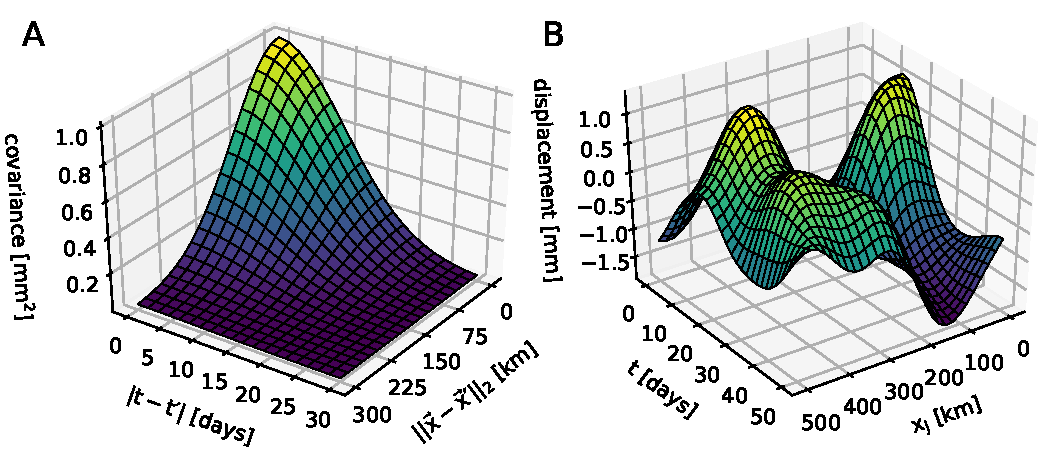
\includegraphics{figures/prior_demo/prior-demo.pdf}
\caption{ 
(A) An example covariance function for transient displacements,
$C_{u_i}(p,p')$, shown as a function of the spatial and temporal
distance between $p$ and $p'$. (B) A single realization of transient
displacements, $u_i(p)$, corresponding to the covariance function from
Panel A. The realization is a function of three variables, $t$,
$x_\mathrm{e}$, and $x_\mathrm{n}$, although we only show its
dependence on $t$ and one of the spatial dimensions.
}    
\label{fig:PriorDemo}
\end{figure*}

% define the components of a datum 

GNSS data records transient displacements as well as other physical
and non-physical processes that we are not interested in. We first
consider component $i$ of a single GNSS displacement observation made
at station $j$, which is located at $\pos^{(j)}$, and time $t^{(k)}$.
We describe this observation, $d_i^{*(jk)}$, as a realization of the
random variable
\begin{align}\label{eq:Data}
\begin{split}
d_i^{(jk)} = &u_i\left(\pos^{(j)},t^{(k)}\right) + 
              \eta_i^{(jk)} + 
              a_i^{(j)} + b_i^{(j)}t^{(k)} + \\
             &c_i^{(j)}\sin\left(2 \pi t^{(k)}\right) +  
              e_i^{(j)}\cos\left(2 \pi t^{(k)}\right) + \\ 
             &f_i^{(j)}\sin\left(4 \pi t^{(k)}\right)  + 
              g_i^{(j)}\cos\left(4 \pi t^{(k)}\right), 
\end{split}
\end{align}
where $\eta_i^{(jk)}$ describes noise, $a_i^{(j)}$ is an offset that
is unique for each station, $b_i^{(j)}$ is the secular velocity at
$\pos^{(j)}$, and the sinusoids describe seasonal deformation (using
units of years for $t^{(k)}$). 

% define the data vector 

We then consider the column vector of $n$ GNSS displacement
observations, $\data^*_i$, where the subscript indicates that we are
still only considering component $i$ of displacements. The
observations are made at $m$ stations, and the times and positions for
each observation are described by the set $\points$. The data vector
$\data^*_i$ can be considered a realization of the random vector
$\data_i$, which is formed by evaluating eq. (\ref{eq:Data}) at each
point in $\points$. To write out $\data_i$ explicitly, we let $\G$ be
an $n \times 6m$ matrix consisting of the basis functions from eq.
(\ref{eq:Data}) (i.e., the linear trends and sinusoids for each
station) evaluated at each point in $\points$. The coefficients
corresponding to each basis function are collected into the column
vector $\mitbf{m}_i$. The noise for all the observations are described
by the column vector $\mitbf{\eta}_i$. We can then write $\data_i$ as
\begin{equation}\label{eq:DataVec}
\data_i = u_i(\points) + \mitbf{\eta}_i + \G\mitbf{m}_i,
\end{equation}
where the notation $u_i(\points)$ represents the column vector
$[u_i(p)]_{p \in \points}$.

% establishing the distribution of the parameters in d and d itself

We assume a diffuse prior for the components of $\mitbf{m}_i$, that is
to say $\mitbf{m}_i \sim \mathcal{N}(\zeros,\kappa^2\eye)$ in the
limit as $\kappa \to \infty$. Of course, the secular velocities,
$b_i^{(j)}$, are spatially correlated and we could invoke a tectonic
model to form a prior on $b_i^{(j)}$. However, in our application to
the Pacific Northwest, we will be using displacement time series which
are long enough to sufficiently constrain $b_i^{(j)}$ for each
station, avoiding the need to incorporate a prior. Likewise, seasonal
deformation is spatially correlated \citep{Dong2002,Langbein2008}, and
it may be worth exploring and exploiting such a correlation in a
future study. We assume that $\mitbf{\eta}_i$ is a spatially and/or
temporally correlated random vector distributed as
$\mathcal{N}(\zeros,\mitbf{C}_{\eta_i})$. For example,
$\mitbf{\eta}_i$ can be uncorrelated white noise, temporally
correlated noise describing benchmark wobble
\citep[e.g.,][]{Wyatt1982,Wyatt1989}, and/or spatially correlated
noise describing common mode error \citep[e.g.,][]{Wdowinski1997}. The
appropriate noise model may vary depending on the application, and we
hold off on specifying the covariance matrix, $\mitbf{C}_{\eta_i}$,
until Section \ref{sec:NoiseModel}. We are now able to write the
distribution of $\data_i$ as
\begin{equation}\label{eq:DataDist}
\data_i \sim \mathcal{N}\left(\zeros, C_{u_i}(\points,\points) + 
                                      \mitbf{C}_{\eta_i}  + 
                                      \kappa^2\G\G^T \right),
\end{equation}
where $C_{u_i}(\points,\points)$ represents the matrix
$[C_{u_i}(p,p')]_{(p,p') \in \points \times \points}$.

% Combining the data and prior to form posterior transient
% displacements

We form a posterior estimate of transient displacements, denoted as
$\post_i$, by updating $u_i$ with the fact that $\data_i^*$ was
realized from the random vector $\data_i$, that is to say $\post_i =
u_i |(\data_i = \data^*_i)$. A general solution for $\post_i$ is
derived in \citet[sec. 8.9]{VonMises1964}, where we find that
$\post_i$ is distributed as $\mathcal{GP}(\mu_{\post_i},C_{\post_i})$
with mean function
\begin{align}\label{eq:PosteriorMean}
\mu_{\post_i}(p) &= \E{u_i(p)} + 
                    \Cov{u_i(p),\data_i} 
                    \Cov{\data_i}^{-1}
                    \left(\data^*_i - \E{\data_i}\right)\nonumber \\
                 &= C_{u_i}(p,\points)\left( C_{u_i}(\points,\points) + 
                                             \mitbf{C}_{\eta_i} + 
                                             \kappa^2\G\G^T\right)^{-1}
                    \data^*_i
\end{align}    
and covariance function
\begin{align}\label{eq:PosteriorCov}
C_{\post_i}(p,p') &= \Cov{u_i(p),u_i(p')} - 
                     \Cov{u_i(p),\data_i} 
                     \Cov{\data_i}^{-1}
                     \Cov{\data_i,u_i(p')} \nonumber \\
                  &= C_{u_i}(p,p') - 
                     C_{u_i}(p,\points)\left( C_{u_i}(\points,\points) + 
                                              \mitbf{C}_{\eta_i} + 
                                              \kappa^2\G\G^T \right)^{-1}
                     C_{u_i}(\points,p').
\end{align}
However, we are interested in the limit as $\kappa \to \infty$, and
the form for eqs. (\ref{eq:PosteriorMean}) and (\ref{eq:PosteriorCov})
is not suitable for evaluating this limit. We use a partitioned matrix
inversion identity \citep[sec. 2.7.4]{Press2007} to rewrite eqs.
(\ref{eq:PosteriorMean}) and (\ref{eq:PosteriorCov}) as
\begin{equation}\label{eq:PosteriorMean2}
\mu_{\post_i}(p) = \left[\begin{array}{cc} 
                         C_{u_i}(p,\points) & \zeros \\
                         \end{array}\right]
                   \left[\begin{array}{cc}
                         C_{u_i}(\points,\points) + \mitbf{C}_{\eta_i} & \G \\
                         \G^T  & -\kappa^{-2} \eye \\
                         \end{array}\right]^{-1}
                   \left[\begin{array}{c}
                         \data^*_i \\
                         \zeros \\
                         \end{array}\right]
\end{equation}    
and
\begin{multline}\label{eq:PosteriorCov2}
C_{\post_i}(p,p') = C_{u_i}(p,p') - \\ 
                    \left[\begin{array}{cc}
                          C_{u_i}(p,\points) & \zeros \\
                          \end{array}\right]
                    \left[\begin{array}{cc}
                          C_{u_i}(\points,\points) + \mitbf{C}_{\eta_i} & \G \\
                          \G^T  & -\kappa^{-2} \eye \\
                          \end{array}\right]^{-1}
                    \left[\begin{array}{c}
                          C_{u_i}(\points,p') \\
                          \zeros \\
                          \end{array}\right].
\end{multline}
Taking the limit as $\kappa \to \infty$, we get the solution for the
mean and covariance of $\post_i$,
\begin{equation}\label{eq:PosteriorMean3}
\mu_{\post_i}(p) = \left[\begin{array}{cc}
                         C_{u_i}(p,\points) & \zeros \\
                         \end{array}\right]
                   \left[\begin{array}{cc}
                         C_{u_i}(\points,\points) + \mitbf{C}_{\eta_i} & \G \\
                         \G^T  & \zeros \\
                         \end{array}\right]^{-1}
                   \left[\begin{array}{c}
                         \data^*_i \\
                         \zeros \\
                         \end{array}\right]
\end{equation}    
and
\begin{equation}\label{eq:PosteriorCov3}
C_{\post_i}(p,p') = C_{u_i}(p,p') - 
                    \left[\begin{array}{cc}
                          C_{u_i}(p,\points) & \zeros \\
                          \end{array}\right]
                    \left[\begin{array}{cc}
                          C_{u_i}(\points,\points) + \mitbf{C}_{\eta_i} & \G \\
                          \G^T  & \zeros \\
                          \end{array}\right]^{-1}
                    \left[\begin{array}{c}
                          C_{u_i}(\points,p') \\
                          \zeros \\
                          \end{array}\right].
\end{equation}
To ensure that the inverse matrices in eqs. (\ref{eq:PosteriorMean3})
and (\ref{eq:PosteriorCov3}) exist, each column in $\G$ must be
linearly independent. This condition tends to be violated when there
are too few observations at a station. In that case, a singular value
decomposition can be used to remove linearly dependent components from
$\G$.

% Noting that we ignore covariance between components

It should be noted that we have ignored any covariances between the
easting and northing components of $\vec{u}$ and $\vec{\data}$.
This simplification reduces the computational complexity of evaluating
the posterior transient displacements because each component can be
evaluated independently. However, we are inherently assuming that the
principle axes describing the distribution of $\vec{u}(p)$ and
$\vec{d}^{(jk)}$ are aligned with the cardinal directions, which is
admittedly an arbitrary assumption.

% converting posterior transient displacements to posterior transient
% strain

The posterior transient displacements are spatially and temporally
continuous, and we can use eqs. (\ref{eq:PosteriorMean3}) and
(\ref{eq:PosteriorCov3}) to evaluate $\post_i$ at any $p$.
Furthermore, $\post_i$ is spatially and temporally differentiable,
allowing us to formulate $\strain$ at any $p$ that we may be
interested in. The components of $\strain$ can be written as
\begin{equation}\label{eq:StrainRate}
\strain_{ij}(p) = \frac{1}{2} \frac{\partial}{\partial t} 
                  \left(\frac{\partial \post_i(p)}{\partial x_j} +  
                        \frac{\partial \post_j(p)}{\partial x_i} \right).
\end{equation}
Since eq. (\ref{eq:StrainRate}) is a linear operation on the Gaussian
processes $\post_i$ and $\post_j$, we know that $\strain_{ij}$ is also
a Gaussian process. From \citet[sec. 10]{Papoulis1991}, we find that
the mean and covariance functions for $\dot{\varepsilon}_{ij}$ are
\begin{align}\label{eq:StrainMean}
\mu_{\strain_{\e\e}}(p) &= \frac{\partial^2 \mu_{\post_\e}(p)}{\partial t \, \partial x_\e} \\
\mu_{\strain_{\n\n}}(p) &= \frac{\partial^2 \mu_{\post_\n}(p)}{\partial t \, \partial x_\n} \\
\mu_{\strain_{\e\n}}(p) &= \frac{1}{2}\frac{\partial}{\partial t}\left(
                                    \frac{\partial \mu_{\post_\e}(p)}{\partial x_\n} + 
                                    \frac{\partial \mu_{\post_\n}(p)}{\partial x_\e} \right)
\end{align} 
and
\begin{align}\label{eq:StrainCov}
C_{\strain_{\e\e}}(p,p') &= \frac{\partial^4 C_{\post_\e}(p,p')}{\partial t \, \partial t' \, \partial x_\e \, \partial x'_\e} \\
C_{\strain_{\n\n}}(p,p') &= \frac{\partial^4 C_{\post_\n}(p,p')}{\partial t \, \partial t' \, \partial x_\n \, \partial x'_\n} \\
C_{\strain_{\e\n}}(p,p') &= \frac{1}{4} \frac{\partial^2}{\partial t \, \partial t'}\left(
                                        \frac{\partial^2 C_{\post_\e}(p,p')}{\partial x_\n \, \partial x'_\n} + 
                                        \frac{\partial^2 C_{\post_\n}(p,p')}{\partial x_\e \, \partial x'_\e} \right),
\end{align} 
respectively. The above derivatives of $\mu_{\post_i}$ and
$C_{\post_i}$ are computed analytically by replacing the terms
$C_{u_i}(p,\points)$, $C_{u_i}(\points,p')$, and $C_{u_i}(p,p')$ in
eqs. (\ref{eq:PosteriorMean3}) and (\ref{eq:PosteriorCov3}) with their
appropriate derivatives. For example, the mean and covariance
functions for $\strain_{\e\e}$ can be written more verbosely as
\begin{equation}\label{eq:StrainMeanEE}
\mu_{\strain_{\e\e}}(p) = \left[\begin{array}{cc}
                          \frac{\partial^2 C_{u_\e}\left( p,\points \right)}{\partial t \, \partial x_\e} & \zeros \\
                          \end{array}\right]
                          \left[\begin{array}{cc}
                          C_{u_\e}(\points,\points) + \mitbf{C}_{\eta_\e} & \G \\
                          \G^T  & \zeros \\
                          \end{array}\right]^{-1}
                          \left[\begin{array}{c}
                          \data^*_\e \\
                          \zeros \\
                          \end{array}\right]
\end{equation}    
and
\begin{multline}\label{eq:StrainCovEE}
C_{\strain_{\e\e}}(p,p') = \frac{\partial^4 C_{u_\e}(p,p')}{\partial t \, \partial t' \, \partial x_\e \, \partial x'_\e} - \\
                           \left[\begin{array}{cc}
                           \frac{\partial^2 C_{u_\e}\left( p,\points \right)}{\partial t \, \partial x_\e} & \zeros \\
                           \end{array}\right]
                           \left[\begin{array}{cc}
                           C_{u_\e}(\points,\points) + \mitbf{C}_{\eta_\e} & \G \\
                           \G^T  & \zeros \\
                           \end{array}\right]^{-1}
                           \left[\begin{array}{c}
                           \frac{\partial^2 C_{u_\e}\left(\points, p' \right)}{\partial t' \, \partial x'_\e} \\
                           \zeros \\
                           \end{array}\right].
\end{multline}    

%% TRANSIENT DETECTION CRITERION
\subsection{Transient detection criterion}\label{sec:TransientDetection}

Our motivation for estimating transient strain rates is, in part, to
detect transient geophysical processes. As we will see, geophysical
signal can be easily identified by visually inspecting the solution
for $\strain$ from eqs. (\ref{eq:StrainMean}) and
(\ref{eq:StrainCov}). However, if we want to detect geophysical signal
automatically, then we need to define a detection criterion. We use a
signal-to-noise ratio, SNR, that is based on the Frobenius norm of
$\strain$, $||\strain||_\mathrm{F} = \left(\strain_{\e\e}^2 +
\strain_{\n\n}^2 + 2\strain_{\e\n}^2\right)^{\frac{1}{2}}$, for our
detection criterion. In the geodetic literature,
$||\dot{\varepsilon}||_\mathrm{F}$ is often used as a metric for the
strain rate ``magnitude", and it is sometimes referred to as the
second invariant of strain rate. Noting that $||\strain||_\mathrm{F}$
is a random variable, we take SNR to be the ratio of the estimated
mean and standard deviation of $||\strain||_\mathrm{F}$. An estimate
of the mean is found by evaluating $||\strain||_\mathrm{F}$ at the
mean of $\strain$,
\begin{align}
\mu_{||\strain||_\mathrm{F}} &\approx ||\strain||_F \big|_{\strain = \mu_{\strain}}\nonumber \\
                             &= \left(\mu_{\strain_{\e\e}}^2 + 
                                      \mu_{\strain_{\n\n}}^2 + 
                                      2\mu_{\strain_{\e\n}}^2 \right)^\frac{1}{2},
\end{align}
and we use nonlinear uncertainty propagation to estimate the standard
deviation,
\begin{equation}
\sigma_{||\strain||_\mathrm{F}} \approx
\left( \left(\left. \frac{\partial ||\strain||_\mathrm{F}}{\partial \strain_{\e\e}}\right|_{\strain = \mu_{\strain}} \right)^2 
       \sigma^2_{\strain_{\e\e}} +
       \left(\left. \frac{\partial ||\strain||_\mathrm{F}}{\partial \strain_{\n\n}}\right|_{\strain = \mu_{\strain}} \right)^2
       \sigma^2_{\strain_{\n\n}} +
       \left(\left. \frac{\partial ||\strain||_\mathrm{F}}{\partial \strain_{\e\n}}\right|_{\strain = \mu_{\strain}} \right)^2 
       \sigma^2_{\strain_{\e\n}} \right)^\frac{1}{2},
\end{equation}
where $\sigma^2_{\strain_{ij}}(p) = C_{\strain_{ij}}(p,p)$. After some
calculations, we find SNR to be
\begin{align}\label{eq:SNR}
\mathrm{SNR}(p) &= \frac{\mu_{||\strain||_\mathrm{F}}(p)}{\sigma_{||\strain||_\mathrm{F}}(p)} \\
                &= \frac{\mu_{\strain_{\e\e}}(p)^2 +
                         \mu_{\strain_{\n\n}}(p)^2 +
                         2\mu_{\strain_{\e\n}}(p)^2}
                        {\big(\sigma^2_{\strain_{\e\e}}(p)\mu_{\strain_{\e\e}}(p)^2 + 
                              \sigma^2_{\strain_{\n\n}}(p)\mu_{\strain_{\n\n}}(p)^2 + 
                              4\sigma^2_{\strain_{\e\n}}(p)\mu_{\strain_{\e\n}}(p)^2
                         \big)^{\frac{1}{2}}}.
\end{align}
We explicitly show that SNR is a function of $p$ to emphasize that it
identifies the position and time of anomalous deformation. We can
reasonably suspect that some transient geophysical phenomena is
occurring wherever and whenever SNR is larger than ${\sim}3$.

%% OUTLIER DETECTION
\subsection{Outlier detection}\label{sec:Outlier}

% Non-technical description of outlier detection methods and our
% outlier detection method

In deriving our formulation for transient strain rates, we have
assumed that noise in the data vector is normally distributed. This is
not an appropriate assumption for GNSS data, which often have more
outliers than would be expected for normally distributed noise.
Methods for analyzing GNSS data should either be robust against
outliers or should involve a preprocessing step in which outliers are
detected and removed. Examples of the former include the MIDAS method
for estimating secular velocities \citep{Blewitt2016} and the GPS
Imaging method for detecting spatially coherent features
\citep{Hammond2016}. In this study, we identify and remove outliers as
a preprocessing step before estimating $\strain$. Outliers are
identified based on the residuals for a model that best fits the
observed data. Observations with residuals that exceed some threshold
are removed. This strategy for detecting outliers is commonly used for
GNSS data, where the model being fit to the data typically consists of
a linear trend and seasonal terms for each GNSS station
\citep[e.g.,][]{Johansson2002,Dong2006,Bos2013}. To prevent transient
geophysical signal from being erroneously identified as outliers, the
model used in our outlier detection algorithm additionally consists of
a temporally correlated Gaussian process. The details of our algorithm
are given in Appendix A.

% Acknowledging that jumps are not detected 

It should be noted that our algorithm does not identify jumps in GNSS
time series, which are another common issue. Some, but not all, jumps
can be automatically removed by looking up the dates of equipment
changes and earthquakes \citep{Gazeaux2013}. However, it is still
necessary to manually find and remove jumps of unknown origin.


%% Application to Pacific Northwest Slow Slip Events
%%%%%%%%%%%%%%%%%%%%%%%%%%%%%%%%%%%%%%%%%%%%%%%%%%%%%%%%%%%%%%%%%%%%%
\section{Application to Pacific Northwest Slow Slip Events}\label{sec:Cascadia}

% Overview of what we are doing in this section

In this section we estimate transient strain rates in the Pacific
Northwest, and we are specifically interested in identifying transient
strain resulting from SSEs \citep[e.g.,][]{Dragert2001}. Before
estimating transient strain rates, we establish a noise model for GNSS
stations in this region, and we establish a prior Gaussian process to
describe displacements from SSEs. SSEs in the Pacific Northwest can be
detected by monitoring for associated seismic tremor
\citep{Rogers2003}, which is actively being done by the Pacific
Northwest Seismic Network \citep{Wech2010}. We can then compare the
tremor records to our estimated transient strain rates to verify that
we are indeed identifying strain from SSEs.

% Dataset used here

We use the daily displacement solutions for continuous GNSS stations
generated by the Geodesy Advancing Geosciences and EarthScope (GAGE)
Facility \citep{Herring2016}. We limit the dataset to the stations and
times that are pertinent to the seven most recent SSEs in the Puget
Sound region. The earliest SSE considered in this study began in
August 2010, and the most recent SSE began in February 2017. The
positions of GNSS stations used to estimate transient strain rates are
shown in Figure \ref{fig:Context}.

\begin{figure*}
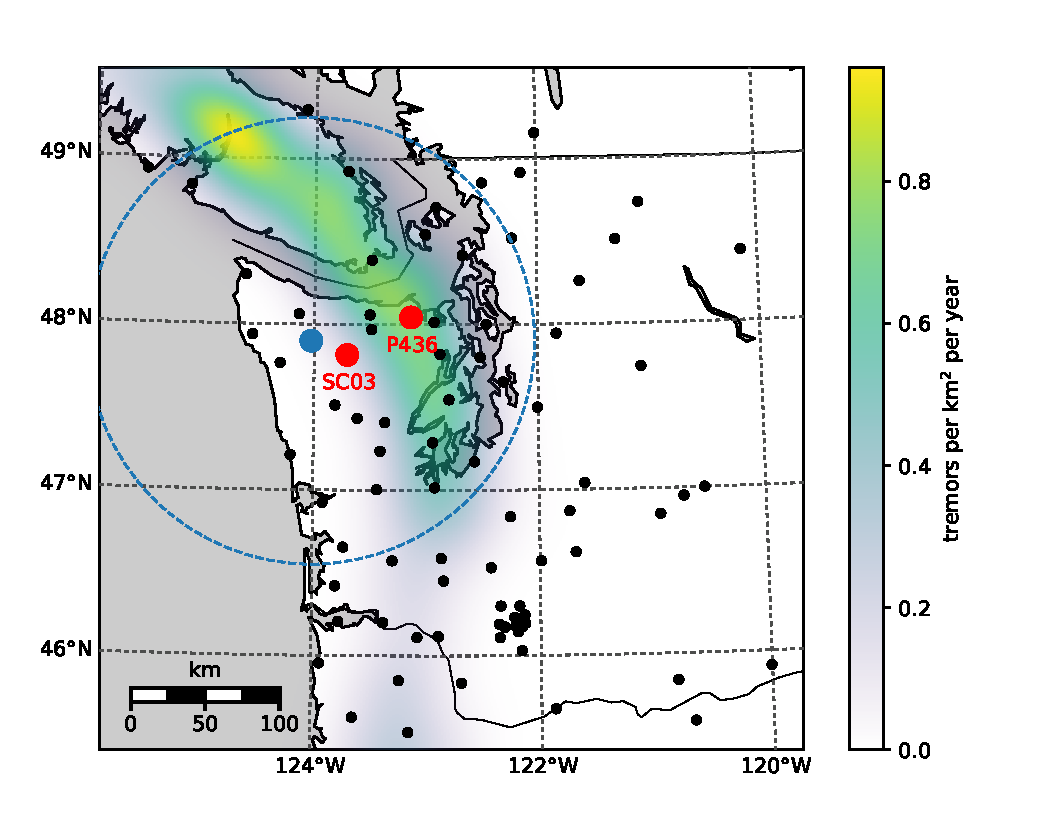
\includegraphics{figures/context_map/context-map.pdf}
\caption{
Positions of the GNSS stations used to estimate transient strain
rates. The colored regions indicate the distribution of seismic tremor
as determined by \citet{Wech2010}. The red dots show the positions of
GNSS stations mentioned in this paper. The blue dot indicates the
location of the transient strain rates shown in Figure
\ref{fig:StrainTs} and the signal-to-noise ratio shown in Figure
\ref{fig:StrainMag}. The blue dashed circle demarcates the spatial
extent of the tremors shown in Figure \ref{fig:StrainMag}.
}    
\label{fig:Context}
\end{figure*}

%% NOISE MODEL
\subsection{Noise model}\label{sec:NoiseModel}

% Defining the components of the noise vector

We consider the noise vector, $\mitbf{\eta}_i$, to be composed of a
temporally correlated Gaussian process, $z_i \sim
\mathcal{GP}(0,C_{z_i})$, and a vector of uncorrelated
Gaussian noise, $\mitbf{w}_i$, so that
\begin{equation}
\mitbf{\eta}_i = z_i(\points) + \mitbf{w}_i.
\end{equation}
The standard deviations for $\mitbf{w}_i$ are taken to be the
uncertainties derived for the GNSS displacement solutions,
$\mitbf{\sigma}_i$. The noise vector then has zero mean and the
covariance matrix
\begin{equation}
\mitbf{C}_{\eta_i} = C_{z_i}(\points,\points) +
                     \mathrm{diag}(\mitbf{\sigma}_i^2).
\end{equation}

% Justifying our temporal noise model

The temporally correlated noise in GNSS data has been thoroughly
studied over the past two decades \citep[e.g.,][]{Zhang1997, Mao1999,
Williams2004, Langbein2008}. In these studies, temporally correlated
noise tends to be described with some combination of Brownian motion
(also known as random walk noise or a Weiner process), a first-order
Gauss-Markov (FOGM) process, and/or flicker noise. There is some
physical justification for using Brownian motion as a noise model
because it accurately describes the power spectrum of motion resulting
from instability in a geodetic monument \citep[e.g.,][]{Wyatt1982,
Wyatt1989}. In particular, the power spectrums for Brownian motion and
monument motion both decay proportionally to $f^{-2}$, where $f$ is
frequency. However, Brownian motion necessarily contains a reference
time at which the process begins. Since there is no notion of when
noise ``begins" in GNSS data, we do not find Brownian motion to be an
appropriate noise model. On the other hand, a FOGM process has no
reference time (i.e., it is stationary), and its power spectrum,
\begin{equation}\label{eq:FOGMPS}
S(f) = \frac{\beta^2}{(2 \pi f)^2 + \alpha^2},
\end{equation}
decays proportionally to $f^{-2}$ above the cutoff frequency $\alpha /
(2 \pi)$. We then choose $z_i$ to be a spatially
uncorrelated FOGM process, which has the covariance function
\begin{equation}\label{eq:FOGM}
C_{z_i}\left((\pos,t),(\pos',t')\right) = 
\frac{\beta^2}{2\alpha}
\exp\left(-\alpha|t - t'|\right)\delta_{\pos,\pos'},
\end{equation}
where $\delta_{\pos,\pos'}$ is 1 if $\pos = \pos'$ and 0 otherwise.
See \citet[sec. B2]{Rasmussen2006} for more information on the FOGM
process.

% How we constrain the parameters

By choosing a FOGM process for $z_i$, we have introduced two
parameters that need to be constrained, $\alpha$ and $\beta$. We
constrain these parameters, which we collectively refer to as
$\mitbf{\theta}$, with the Restricted Maximum Likelihood (REML) method
\citep{Harville1974}. The REML method is conceptually similar to the
Maximum Likelihood Estimation (MLE) method from \citet{Langbein1997},
where we pick $\mitbf{\theta}$ to maximize the probability of drawing
the observed data, $\mitbf{d}_i^*$, from the random vector
$\mitbf{d}_i$. However, unlike the MLE method, the REML method
produces unbiased estimates of $\mitbf{\theta}$ \citep[sec.
2.6]{Cressie1992}. We use the REML method to estimate $\mitbf{\theta}$
at 38 continuous GNSS stations in the Pacific Northwest that are east
of 121$^\circ$W. These stations are sufficiently far from the
subduction zone that they are unlikely to record transient deformation
from SSEs, allowing us to ingore the term $u_i(\points)$ in
$\mitbf{d}_i$. We assume the noise at these inland stations is
representative of the noise at all the stations considered in this
study, which is probably a poor assumption since the inland stations
are subject to distinctly different climatic conditions. Nonetheless,
we find $\mitbf{\theta}$ for each of the inland stations and for each
displacement component by maximizing the REML likelihood function
\begin{equation}\label{eq:REMLNoise}
\mathcal{L}(\mitbf{\theta}) = \left(\frac{\left|\G^T\G\right|}{(2\pi)^{n-6m} 
                                    \left| \mitbf{C}_{\eta_i}(\mitbf{\theta}) \right| 
                                    \left| \G^T\mitbf{C}_{\eta_i}(\mitbf{\theta})^{-1}\G \right|}\right)^{\frac{1}{2}} 
                              e^{-\tfrac{1}{2}\data_i^{*T}\mitbf{K}(\mitbf{\theta})\data_i^*}
\end{equation}
with respect to $\mitbf{\theta}$, where
\begin{equation}
\mitbf{K}(\mitbf{\theta}) = \mitbf{C}_{\eta_i}(\mitbf{\theta})^{-1} - 
                            \mitbf{C}_{\eta_i}(\mitbf{\theta})^{-1}\G
                            \left(\G^T\mitbf{C}_{\eta_i}(\mitbf{\theta})^{-1}\G\right)^{-1}
                            \G^T\mitbf{C}_{\eta_i}(\mitbf{\theta})^{-1}.
\end{equation}
In the above equation, $\data^*_i$ consists of the data for a single station.

% results of estimated parameters

The distribution of inferred values for $\alpha$ and $\beta$ are shown
in Figure \ref{fig:NoiseParams}. The estimates of $\beta$ for the
easting and northing components are clustered around 0.5
mm/yr$^{0.5}$. The corresponding estimates of $\alpha$ tend to cluster
around 0 yr$^{-1}$, indicating that the power spectrum of noise indeed
decays proportionally to $f^{-2}$ over a wide band of frequencies. We
also estimate $\alpha$ and $\beta$ for the vertical component of
displacements, with the hope that vertical deformation gradients could
reveal some geophysical signal. For the vertical component, $\beta$ is
relatively large with a median value of 13.5 mm/yr$^{0.5}$. The
inferred values for $\alpha$ are also higher for the vertical
component with a median value of 8.21 yr$^{-1}$. In Figure
\ref{fig:NoiseSamples}, we use the median values of $\alpha$ and
$\beta$ to generate two realizations of FOGM noise for each component.
The realizations span five years, and the easting and northing
realizations drift by about 1 mm over these five years. In the context
of detecting SSEs, which produce several mm's of surface displacement
on the time-scale of weeks, the estimated FOGM noise for the easting
and northing component is negligible. In contrast, the estimated FOGM
noise for the vertical component is larger than the signal we would
expect from SSEs. We suspect that the higher amplitude for the FOGM
noise in the vertical component is accommodating for deficiencies in
our rather simple seasonal model. Based on this analysis, we
henceforth ignore temporally correlated noise in the easting and
northing component because of its low amplitude. We also do not use
vertical displacements because of the presumably low signal-to-noise
ratio.

\begin{figure*}
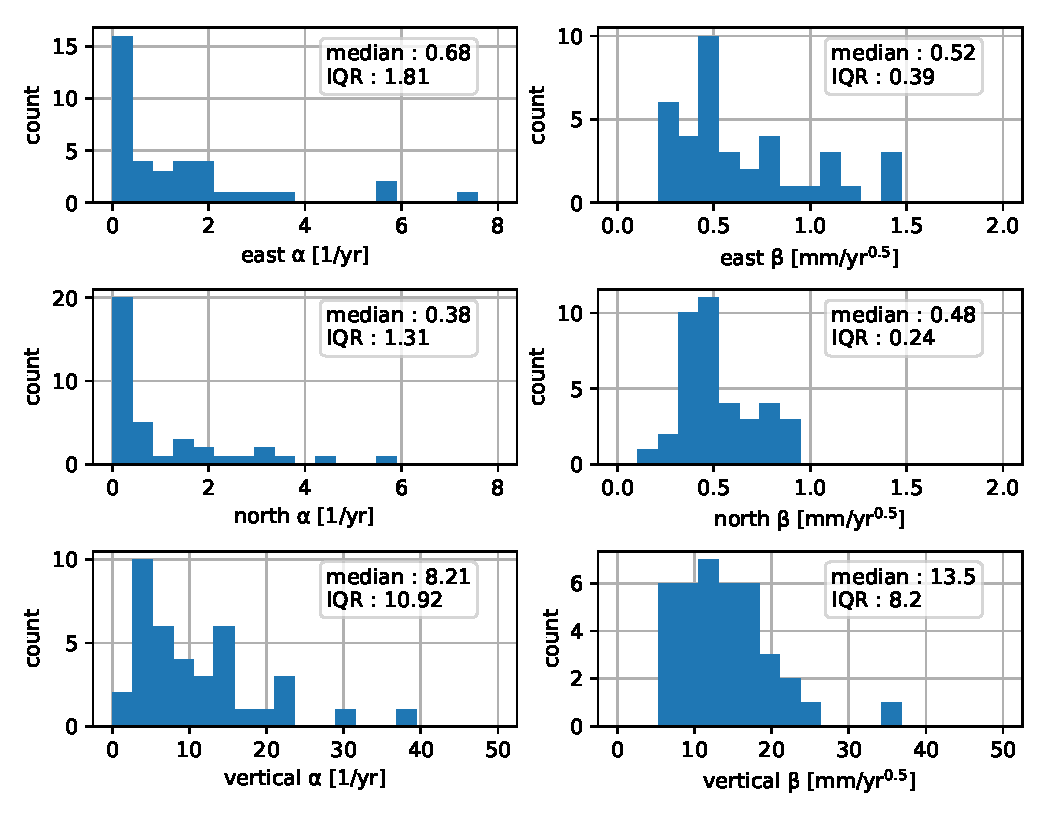
\includegraphics{figures/noise/noise-params.pdf}
\caption{
Distribution of inferred values for the parameters in the FOGM noise
model (eq. \ref{eq:FOGM}). ``IQR'' is the interquartile range of
inferred values.
}   
\label{fig:NoiseParams}
\end{figure*}

\begin{figure*}
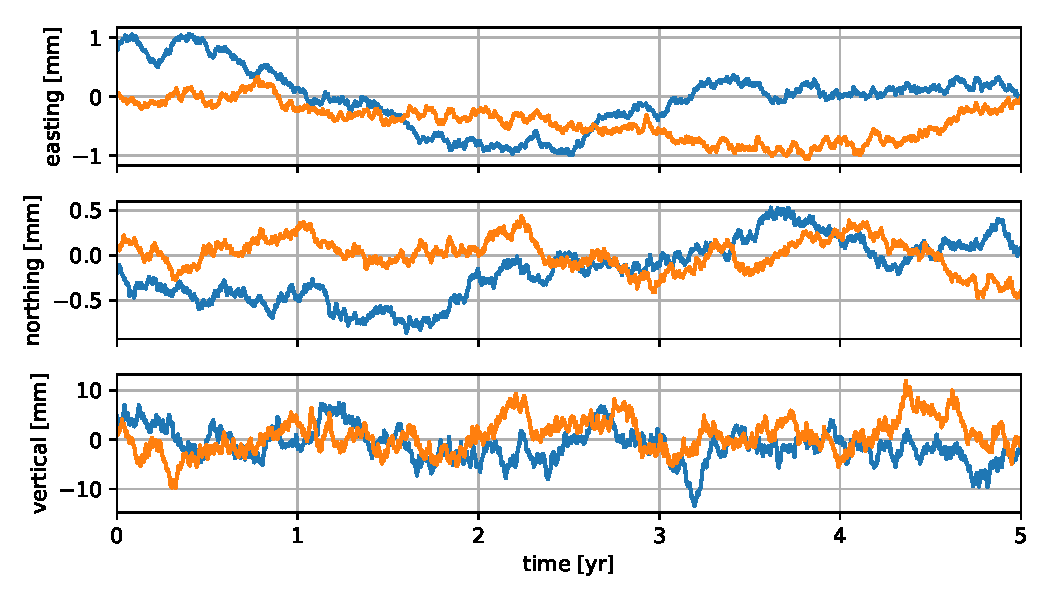
\includegraphics{figures/noise/noise-samples.pdf}
\caption{
Two samples of FOGM noise for each displacement component. The
parameters for the FOGM noise model have been set to the median values
from Figure \ref{fig:NoiseParams}.
}   
\label{fig:NoiseSamples}
\end{figure*}

% Note spatially correlated noise

Another significant source of noise in GNSS data is common mode error
\citep[e.g.,][]{Wdowinski1997,Dong2006}, which is noise that is highly
spatially correlated. When not accounted for, common mode error
manifests as spatially uniform undulations in our estimated transient
displacements. These undulations have no effect on the transient
strain rates, and so we do not need to include common mode error in
our noise model.

%% PRIOR MODEL
\subsection{Prior model}\label{sec:SignalModel}

% State our choice for X_i

We next establish a prior model for transient displacements.
Specifically, we discuss our choice for the spatial and temporal
functions making up $C_{u_i}$, $X_i$ and $T_i$. For $X_i$, we use the
squared exponential (SE) covariance function,
\begin{equation}\label{eq:SE}
X_i(\pos,\pos') = \exp\left(\frac{-||\pos - \pos'||_2^2}{2 \ell^2}\right).
\end{equation}
The SE covariance function is commonly used for kriging
\citep[e.g,][]{Cressie1992} and Gaussian process regression
\citep[e.g.,][]{Rasmussen2006}. In terms of geodetic applications,
\citet{Kato1998} and \cite{El-Fiky1999} demonstrated that the SE
covariance function accurately describes the spatial covariance of
secular GNSS derived velocities in Japan.

% List our choices for T_i

We consider three potential choices for $T_i$. The first option is the
one-dimensional SE covariance function,
\begin{equation}\label{eq:TimeSE}
T_i(t,t') = \phi^2\exp\left(\frac{-|t - t'|^2}{2\tau^2}\right).
\end{equation}
Note that $T_i$ includes the parameter $\phi$, which serves to scale
the covariance function $C_{u_i}$. The second option is a member of
the Wendland class of covariance functions \citep{Wendland2005}.
Wendland covariance functions have compact support and hence their
corresponding covariance matrices are sparse. In our analysis, we
exploit this sparsity with the CHOLMOD software package
\citep{Chen2008}. Wendland covariance functions can be constructed
such that they are positive definite in $\mathbb{R}^d$ and their
corresponding Gaussian process can be differentiated $k$ times. We use
$d=1$, because we are describing the temporal covariance of $u_i$, and
we use $k=2$, giving samples of $u_i$ continuous velocities and
accelerations. The corresponding Wendland covariance function is
\begin{equation}\label{eq:Wendland} 
T_i(t,t') = \phi^2\left(1 - \frac{|t - t'|}{\tau}\right)^5_+ 
            \left(\frac{8|t - t'|^2}{\tau^2} + \frac{5|t - t'|}{\tau} + 1\right), 
\end{equation} 
where $(t)_+ = \mathrm{max}(0,t)$. The third option for $T_i$ is the
covariance function for integrated Brownian motion (IBM). IBM is a
Gaussian process with zero mean and its covariance function can be
found by integrating the covariance function for Brownian motion,
\begin{align}\label{eq:IBM}
T_i(t,t') &= \int_0^t \int_0^{t'} \phi^2 \min(s,s') \,ds'\,ds \\
          &= \frac{\phi^2}{2}\min(t,t')^2 \left(\max(t,t') - \frac{1}{3}\min(t,t')\right), \ \ \ t,t' \geq 0.
\end{align}
IBM has been used in the context of Kalman filtering as a
non-parametric model for the time dependence of geophysical signals
\citep[e.g.,][]{Segall1997, McGuire2003, Ohtani2010, Hines2016a}.
Similar to Brownian motion, IBM has a reference time, $t=0$, at which
the process begins. For some geophysical signals, it is appropriate to
have this reference time. For example, if we are trying to identify
postseismic deformation then $t$ should be zero at the time of the
earthquake.  However, if we are interested in detecting transient
events, where there is no known start time, then IBM may not be an
appropriate prior model. Instead, one may prefer to use the SE or
Wendland covariance functions because they are stationary. In the
following analysis, we make the choice that $t$ is zero on the first
epoch of $\data_i^*$. Using an earlier reference time does not change
the results discussed in this section.

% Choosing the parameters

We use the REML method to determine the appropriate values for the
parameters in $C_{u_i}$, which are $\ell$, $\phi$, and $\tau$. We
refer to these parameters collectively as $\mitbf{\theta}$. Just as in
Section \ref{sec:NoiseModel}, we pick $\mitbf{\theta}$ to maximize the
probability of drawing $\data_i^*$ from $\data_i$, but now we are
including $u_i(\points)$ in $\data_i$. and we are optimizing the
parameters for $C_{u_i}$ rather than $\mitbf{C}_{\eta_i}$. We divide
the GNSS data into seven subsets that are four months long and each
centered on the time of a SSE. The times of the seven SSEs are
determined with tremor records from \cite{Wech2010}. We find the
optimal $\mitbf{\theta}$ for each subset of data, for each
displacement component, and for each choice of $T_i$. The REML
likelihood function that we are maximizing with respect to
$\mitbf{\theta}$ is now
\begin{equation}\label{eq:REMLPrior} 
\mathcal{L}(\mitbf{\theta}) =
\left(\frac{\left| \G^T \G \right|}{(2\pi)^{n-6m}
                                    \left| \mitbf{\Sigma}(\mitbf{\theta}) \right| 
                                    \left| \G^T \mitbf{\Sigma}(\mitbf{\theta})^{-1} \G \right|}\right)^{\frac{1}{2}} 
                              e^{-\tfrac{1}{2} \data_i^{*T} \mitbf{K}(\mitbf{\theta}) \data_i^*},
\end{equation}
where
\begin{equation}
\mitbf{K}(\mitbf{\theta}) = \mitbf{\Sigma}(\mitbf{\theta})^{-1} - 
                            \mitbf{\Sigma}(\mitbf{\theta})^{-1} \G
                            \left( \G^T \mitbf{\Sigma}(\mitbf{\theta})^{-1} \G \right)^{-1}
                            \G^T \mitbf{\Sigma}(\mitbf{\theta})^{-1}
\end{equation}
and $\mitbf{\Sigma}(\mitbf{\theta}) = \mitbf{C}_{\eta_i} +
C_{u_i}(\points,\points;\mitbf{\theta})$. In the above equation,
$\data^*_i$ consists of a single subset of data. The estimated
parameters are summarized in Table 1. Based on the interquartile
ranges, the estimated parameters for the SE and Wendland covariance
functions do not vary significantly between SSEs. This suggests that
the median of the estimated parameters should be appropriate for all
the Pacific Northwest SSEs. For the IBM model, there are several
anomalously large values for $\ell$ and $\phi$, which is why the
interquartile ranges are large.

\begin{table}\label{tab:Parameters}
\caption{
Optimal values for the parameters in $X_i$ and $T_i$ determined with
the REML method. The covariance function for $T_i$ is indicated by the
``$T_i$'' column. The SE, Wendland, and IBM covariance functions are
defined in eqs. (\ref{eq:TimeSE}), (\ref{eq:Wendland}), and
(\ref{eq:IBM}), respectively. We use eq. (\ref{eq:SE}) for $X_i$.
The parameters are estimated for each of the seven SSEs considered in
this study, and the tabulated values indicate the median and
interquartile ranges of estimated values. The ``diff $\log$(REML)'' column
compares the optimal log REML likelihoods to those for when $T_i$ is
the SE covariance function. Negative values indicate that observations
are more consistent with the SE covariance function.
} 
\begin{tabular} {l l l l l l}
$T_i$ & component & $\ell$  & $\phi$   & $\tau$  & diff. $\log$(REML) \\ \hline
SE & east   & 92 $\pm$ 25 km  & 0.62 $\pm$ 0.11 mm  & 0.026 $\pm$ 0.011 yr  &  - \\
SE & north  & 91 $\pm$ 53 km  & 0.43 $\pm$ 0.05 mm  & 0.030 $\pm$ 0.017 yr  &  - \\
Wendland & east   & 95 $\pm$ 30 km  & 0.66 $\pm$ 0.15 mm  & 0.093 $\pm$ 0.044 yr &  0.78 $\pm$ 0.87 \\
Wendland & north  & 92 $\pm$ 57 km  & 0.46 $\pm$ 0.10 mm  & 0.116 $\pm$ 0.057 yr &  0.08 $\pm$ 0.58 \\
IBM & east   & 110 $\pm$ 130 km & 290 $\pm$ 420 mm/yr$^{1.5}$  & -          & -16.4 $\pm$ 7.8 \\
IBM & north  & 150 $\pm$ 560 km & 110 $\pm$ 250 mm/yr$^{1.5}$ & -           & -10.1 $\pm$ 2.3 \\
\end{tabular}
\end{table}

% Choosing the covariance function for T_i with REML

Next, we identify which covariance function for $T_i$ best describes
the time dependence of deformation from SSEs. One approach is to
choose the covariance function that produces the largest optimal REML
likelihoods, similar to the analysis in \citet{Langbein2004}. In Table
1, we summarize how the optimal REML likelihoods for the Wendland and
IBM covariance functions compare to those for the SE covariance
function. Based on the differences in optimal REML likelihoods, the
data is substantially more likely to come from a Gaussian process with
a SE or Wendland covariance function than an IBM covariance function.
The REML likelihoods do not definitively indicate whether the SE or
Wendland covariance function is preferable.

% Choosing the covariance function for T_i with posterior fit

A more intuitive way of deciding which function to use for $T_i$ is to
compare the posterior displacements and the observed displacements.
The posterior displacements consist of our estimate of transient
displacements, secular trends, and seasonal deformation. Specifically,
the posterior displacement vector is $\hat{\data}_i = \left(
u_i(\points) + \G\mitbf{m}_i \right) | \left( \data_i = \data_i^*
\right)$. Following a similar procedure as in Section
\ref{sec:Method}, it can be shown that $\hat{\data}_i$ has a
multivariate normal distribution with mean vector
\begin{equation}\label{eq:DataPredMean}
\mitbf{\mu}_{\hat{d}_i} = \left[\begin{array}{cc}
                          C_{u_i}(\points,\points) & \G \\
                          \end{array}\right]
                          \left[\begin{array}{cc}
                          \mitbf{C}_{\eta_i} + C_{u_i}(\points,\points) & \G \\
                          \G^T  & \zeros \\
                          \end{array}\right]^{-1}
                          \left[\begin{array}{c}
                          \data_i^* \\
                          \zeros \\
                          \end{array}\right]
\end{equation}  
and covariance matrix
\begin{equation}\label{eq:DataPredCov}
\mitbf{C}_{\hat{d}_i} = C_{u_i}(\points,\points) - 
                        \left[\begin{array}{cc}
                              C_{u_i}(\points,\points) & \G \\
                              \end{array}\right]
                        \left[\begin{array}{cc}
                              \mitbf{C}_{\eta_i} + C_{u_i}(\points,\points) & \G \\
                              \G^T  & \zeros \\
                              \end{array}\right]^{-1}
                        \left[\begin{array}{c}
                              C_{u_i}(\points,\points) \\
                              \G^T \\
                              \end{array}\right].
\end{equation}
We compute $\hat{\data}_i$ using the SE, Wendland, and IBM covariance
functions for $T_i$, and we use the median values from Table 1 for
$\mitbf{\theta}$. Figure \ref{fig:Fit} compares $\data_i^*$ to
$\hat{\data}_i$ during the winter 2015-2016 SSE at stations ALBH,
P436, and SC02, which are the stations that recorded the strongest
signal from this SSE. Based on Figure \ref{fig:Fit}, the chosen
covariance function for $T_i$ has almost no effect on $\hat{\data}_i$.
The posterior displacements for the IBM covariance function contain
slightly more high frequency, and perhaps spurious, features.
Regardless of the chosen covariance function, $\hat{\data}_i$ appears
to underestimate the rate of deformation during the SSE at stations
ALBH and SC02. The deformation at these two stations is particularly
rapid compared to the surrounding stations, and the misfit between
$\data_i^*$ and $\hat{\data}_i$ is likely due to over-smoothing. This
over-smoothing could indicate that the chosen values for $\tau$ or
$\ell$ are too large. However, $\hat{\data}_i$ does faithfully fit
$\data_i^*$ at the remaining stations, and so we do not attempt to
further refine the parameters.

% The choice 

For our estimates of transient strain discussed in the next section,
we ultimately settle on the Wendland covariance function for $T_i$,
and we use the median values from Table 1 for the parameters. We
choose the Wendland covariance function over the SE covariance
function because of its computational advantages.

\begin{figure*}
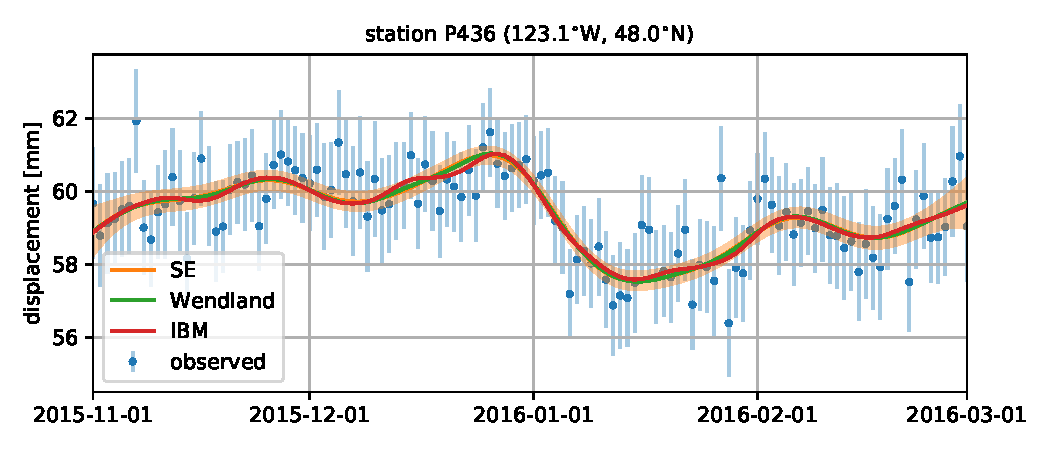
\includegraphics{figures/signal_fit/signal-fit.pdf}
\caption{
Easting component of the observed displacements, $\data_\e^*$, and
posterior displacements, $\hat{\data}_\e$, during the winter 2015-2016
SSE. We show $\hat{\data}_\e$ for when $T_i$ is a SE, Wendland, and
IBM covariance function. The one standard deviation uncertainties are
shown for $\data_\e^*$ and the $\hat{\data}_\e$ that has a SE
covariance function for $T_i$. For clarity, uncertainties are not
shown for the $\hat{\data}_\e$ that have an IBM or Wendland covariance
function for $T_i$. The posterior displacements for the different
covariance functions are all practically indistinguishable.
}   
\label{fig:Fit}
\end{figure*}

%% TRANSIENT STRAIN RATES
\subsection{Transient Strain Rates}\label{sec:Results} 

% Stating how we calculate strain and refering to the figures

Having established a noise model and a prior for transient
displacements, we can now calculate transient strain rates, $\strain$,
in the Puget Sound region from the GNSS data. We evaluate $\strain$ at
a grid of points spanning the study area for each day from January 1,
2010 to May 15, 2017. In Figure \ref{fig:StrainMap}, we show a map
view of $\strain$ on January 1, 2016, which coincides with the height
of the winter 2015-2016 SSE. In Figure \ref{fig:StrainTs}, we show a
time series of $\strain$ at a position on the Olympic Peninsula, which
is where $\strain$ tends to be the largest during SSEs. We also
include a supplementary animation showing a map view of $\strain$ over
time. In each figure, we show the mean and standard deviation of
$\strain$, making it easy to identify which features are statistically
significant.

% Describe the strain during SSEs and tectonic implications

The transient strain rates shown for the winter 2015-2016 SSE in
Figure \ref{fig:StrainMap} are characteristic of most SSEs in the
Puget Sound region. The SSEs cause trench perpendicular compression in
the Olympic Peninsula and extension east of Puget Sound. The strain
transitions from compression to extension around the southern tip of
Vancouver Island, coinciding with where fault slip tends to be
inferred \citep[e.g.,][]{Dragert2001, Wech2009, Schmidt2010}. Thus,
this pattern of strain is to be expected. Over decadal timescales,
there is trench perpendicular compression throughout this study region
caused by steady tectonic plate motion \citep{Murray2000,
McCaffrey2007, McCaffrey2013}. When comparing the transient strain
rates caused by SSEs to the secular strain rates, we see that SSEs are
concentrating tectonically accumulated strain energy towards the
trench, and presumably pushing the subduction zone closer to failure.

\begin{figure*}
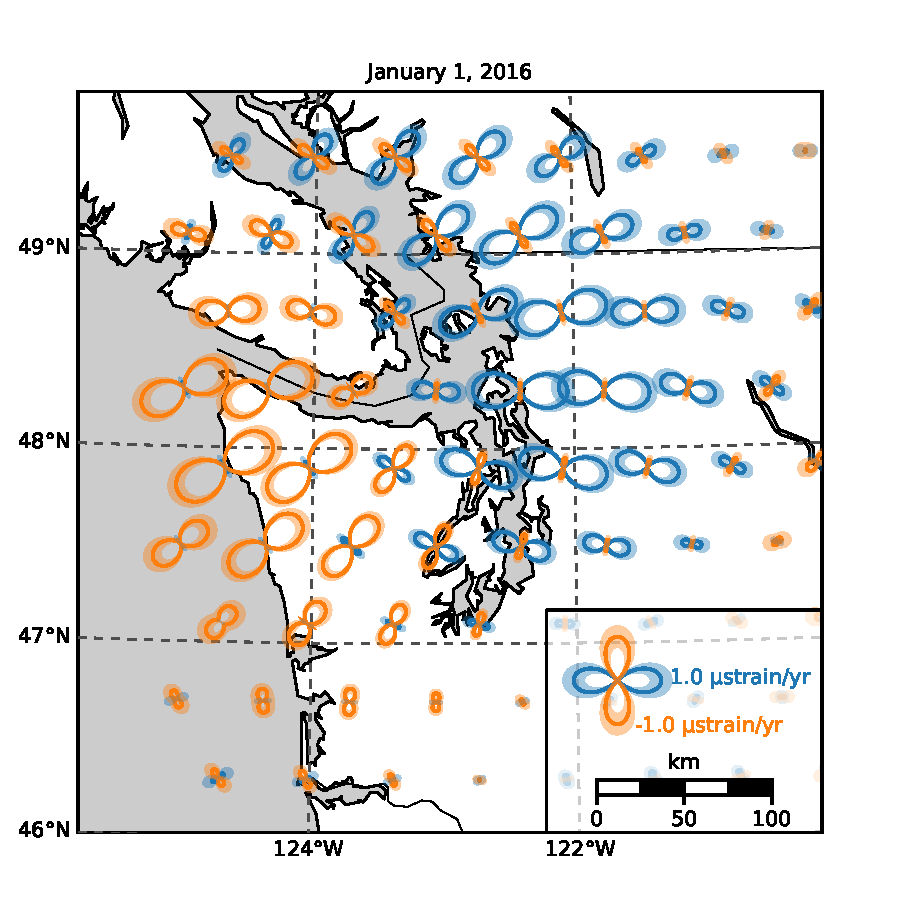
\includegraphics{figures/strain_map/strain-map.pdf}
\caption{
Transient strain rates during the Winter 2015-2016 SSE. The glyphs
show the normal strain rates as a function of azimuth, where orange
indicates compression and blue indicates extension. The shaded regions
indicate the one standard deviation uncertainties for the normal
strain rates.
}   
\label{fig:StrainMap}
\end{figure*}

% compare seismic tremor to SNR

To verify that the estimated transient strain rates are accurately
identifying geophysical signal, we compare the signal-to-noise ratio
from eq. (\ref{eq:SNR}) at a point on the Olympic Peninsula to the
frequency of seismic tremor (Figure \ref{fig:StrainMag}). A
signal-to-noise ratio greater than ${\sim}3$ can be interpreted as a
detected geophysical signal. We detect nine distinct events, which
each correspond to peaks in seismic tremor. The smaller events
detected in August 2014 and February 2017 can be considered inter-SSE
events. They were not among the SSEs used to constrain the prior
covariance function. In between peaks in seismic tremor, the
signal-to-noise ratio is consistently between 0 and 2, suggesting that
all the transient strain detected at this point on the Olympic
Peninsula is associated with SSEs and inter-SSE events.

\begin{figure*}
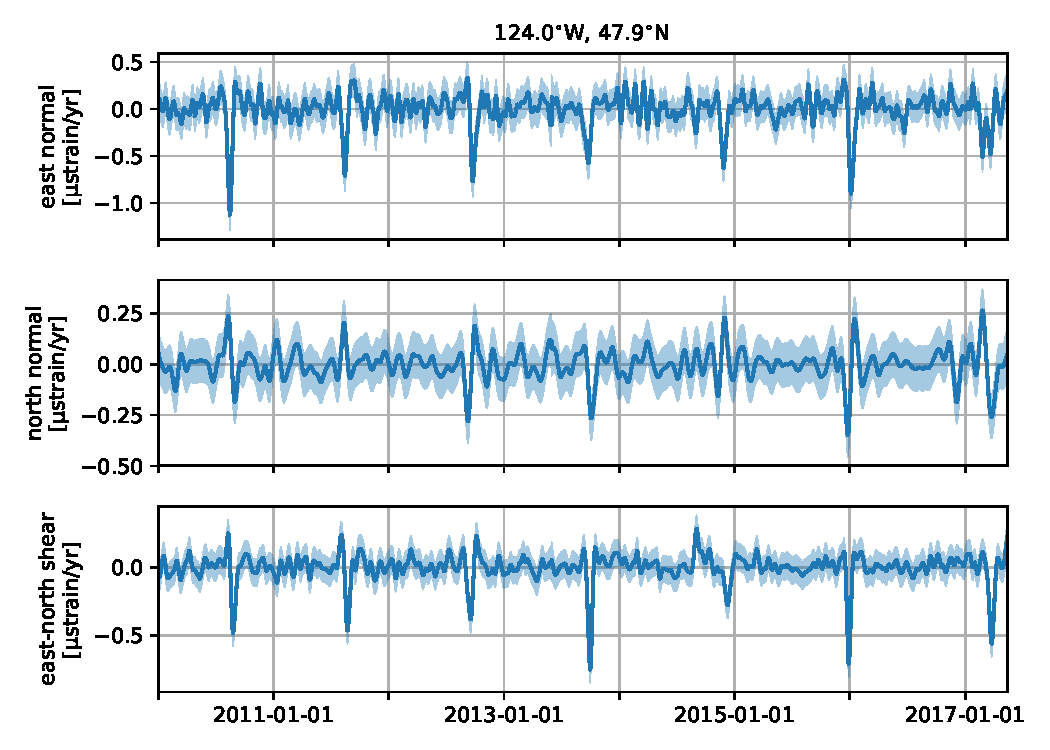
\includegraphics{figures/strain_ts/strain-ts.pdf}
\caption{
Components of the transient strain rates at the position shown in
Figure \ref{fig:Context}. The shaded regions indicate the one standard
deviation uncertainties.
}   
\label{fig:StrainTs}
\end{figure*}

\begin{figure*}
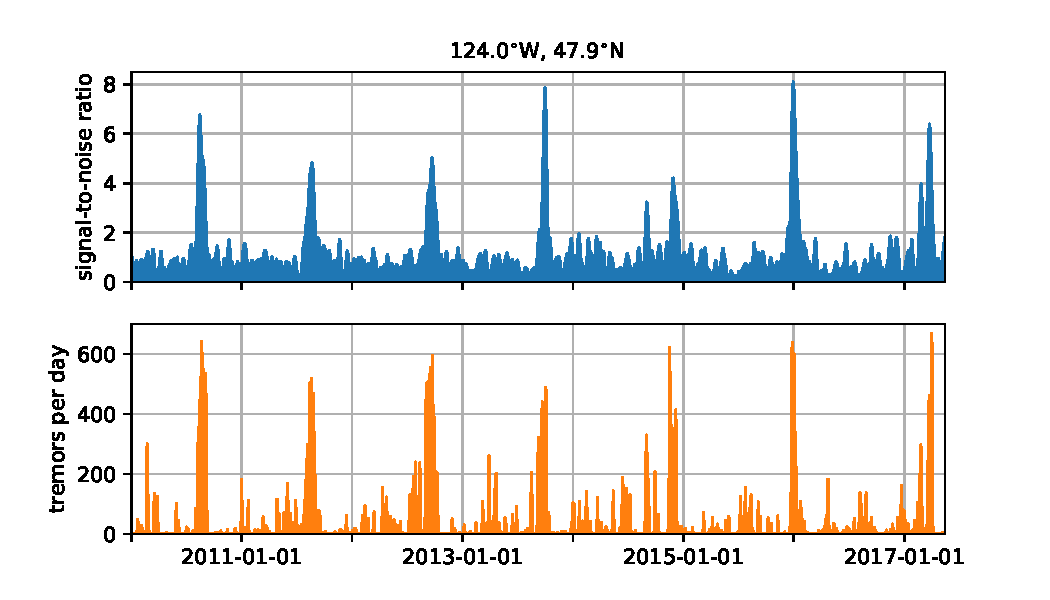
\includegraphics{figures/strain_ts/mag-ts.pdf}
\caption{
(top) Signal-to-noise ratio (eq. \ref{eq:SNR}) at the position shown
in Figure \ref{fig:Context}. (bottom) Frequency of seismic tremors in
the region shown in Figure \ref{fig:Context}.
}   
\label{fig:StrainMag}
\end{figure*}

% note that we are only discussing strain with known origin

The results we have presented indicate that we are identifying the
transient strain that we should expect to see. This is not to say that
there are no unexpected features in $\strain$ that are worth further
exploration. However, a discussion on features in $\strain$ that have
unknown origin would be outside the scope of this paper.

%% DISCUSSION
%%%%%%%%%%%%%%%%%%%%%%%%%%%%%%%%%%%%%%%%%%%%%%%%%%%%%%%%%%%%%%%%%%%%%
\section{Discussion}\label{sec:Discussion}

%% Areas for improvement and further study
% noise model

Our results demonstrate that GPR is an effective tool for estimating
transient strain rates and detecting geophysical processes from GNSS
data. However, there are some aspects of our method that warrant
further research. For example, there is potential for a more thorough
analysis of the spatio-temporal noise in the GNSS data than what was
performed in Section \ref{sec:NoiseModel}. Specifically, we did not
explore spatially correlated noise, such as common mode error. We
have assumed that any spatially correlated noise has a sufficiently
long wavelength that it has a negligible effect on transient strain
rates. We can also improve upon the seasonal noise model used in this
study, which consists of four sinusoids for each station. We did not
explore the roughness of the seasonal deformation (i.e., the number of
sinusoids needed to describe the deformation). The periodic Gaussian
process \citep{Mackay1998} is an alternative model for seasonal
deformation and is well suited for exploring the roughness of seasonal
deformation.  The periodic Gaussian process has zero mean and the
covariance function
\begin{equation}\label{eq:Periodic}
  T(t,t') = \phi^2 \exp\left(\frac{-\sin(\pi|t - t'|)^2}{2\tau^2}\right). 
\end{equation}
Realizations have annual periodicity and the roughness is controlled
by $\tau$. Decreasing $\tau$ has the same effect as including higher
frequency sinusoids in the seasonal model. The optimal value for
$\tau$ can be found with the REML method.

% issues and potential improvements on numerical consideratiosn

% Numerical considerations

% note that the compact covariance function is not a perfect solution
% because it is only compact if the signal has a short timescale. Long
% wavelength features will still have a dense covariance matrix. This is
% part of the reason why we omitted the temporal noise model.

% numerical issues

Another potential research direction would be to reduce the
computational cost of our method for estimating transient strain
rates. GPR is generally computationally expensive when there are many
observations. The transient strain rates estimated in this study are
constrained by seven years of daily displacement observations from 94
GNSS stations, which amounts to about 240,000 observations for each
displacement component. For a dataset with this size, it is difficult
to evaluate the matrix inverses in eqs. (\ref{eq:PosteriorMean3}) and
(\ref{eq:PosteriorCov3}). We alleviate this computational cost by
using a compact Wendland covariance function for our prior. By using a
compact covariance function for our prior, eqs.
(\ref{eq:PosteriorMean3}) and (\ref{eq:PosteriorCov3}) become sparse
systems of equations that are more tractable to evaluate. However, the
sparsity decreases when the Wendland covariance function has a larger
time-scale parameter. The Wendland covariance then offers less of a
computational advantage when we were interested in geophysical
processes that occur over longer times-scales. An alternative approach
to dealing with large datasets would be to explore approximation
methods for GPR \citep[sec. 8]{Rasmussen2006}.

% additional applications

In addition to detecting geophysical processes, the GNSS derived
transient strain rates can be used to better understand the data from
borehole strain meters (BSMs). The Plate Boundary Observatory contains
about forty BSMs in the Pacific Northwest, and it has been
demonstrated that BSMs are able to record transient geophysical events
such as SSEs \citep[e.g.,][]{Dragert2011}. However, there are
complications that prevent BSM data from being used quantitatively in
geophysical studies. One difficulty is that BSM data should be
calibrated with a well known strain source, such as diurnal and
semidiurnal tides \citep{Hart1996,Roeloffs2010,Hodgkinson2013}.
Unfortunately, the tidal forces at BSMs which record SSEs are strongly
influenced by local bodies of water such as the Straight of Juan de
Fuca, making it difficult to form a theoretical prediction of tidal
strains \citep{Roeloffs2010}. Another complication is that noise in
BSM data is not well understood. The noise consists, in part, of a
long-term decay resulting from the instrument equilibrating with the
surrounding rock \citep{Gladwin1987}. Typically, this noise is dealt
with in an ad-hoc manner by fitting and removing exponentials and
low-order polynomials. We envision that the GNSS derived strain rates
from this paper can be used as a reference strain for calibrating BSM
data and quantify its noise.


%% CONCLUSION
%%%%%%%%%%%%%%%%%%%%%%%%%%%%%%%%%%%%%%%%%%%%%%%%%%%%%%%%%%%%%%%%%%%%%
\section{Conclusion}\label{sec:Conclusion}

We propose using Gaussian process regression (GPR) to estimate
transient strain rates from GNSS data. Most other methods for
estimating strain rates assume a parametric representation of
deformation, which can bias the results if the parameterization is not
chosen carefully. Here we assume a stochastic, rather than parametric,
prior model for displacements. Our prior model describes how much we
expect transient displacements to covary spatially and temporally. If
we know nothing about the underlying signal that we are trying to
recover, then the prior model can be chosen objectively with maximum
likelihood methods. We demonstrate that GPR is an effective tool for
detecting geophysical processes, such as slow slip events, in our
application to the Pacific Northwest. While this paper just focuses on
using GPR to estimate transient strain rates and detect geophysical
processes, we believe that GPR is a powerful tool that can be applied
to a wide range of geophysical problems.

%% ACKNOWLEDGEMENTS
%%%%%%%%%%%%%%%%%%%%%%%%%%%%%%%%%%%%%%%%%%%%%%%%%%%%%%%%%%%%%%%%%%%%%
\section{Acknowledgements}
This material is based upon work supported by the National Science
Foundation under grant EAR 1245263. The EarthScope Plate Boundary
Observatory data is provided by UNAVCO through the GAGE Facility with
support from the National Science Foundation (NSF) and National
Aeronautics and Space Administration (NASA) under NSF Cooperative
Agreement EAR-1261833. An implementation of the method described in
this paper is named Python-based Geodetic Network Strain software
(PyGeoNS). PyGeoNS is distributed under the MIT License and can be
found at www.github.com/treverhines/PyGeoNS.

%% APPENDIX
%%%%%%%%%%%%%%%%%%%%%%%%%%%%%%%%%%%%%%%%%%%%%%%%%%%%%%%%%%%%%%%%%%%%%
\appendix
\section{Outlier detection algorithm}

Our outlier detection algorithm is loosely based on the data editing
algorithm from \citet{Acheson1975}. Let $\data^*$ denote all $n$ GNSS
displacement observations for a single directional component, which
have been made at positions and times $\points$.  We describe
$\data^*$ as a realization of the random vector
\begin{equation}\label{eq:OutlierDataVec}
\data = \G\mitbf{m} + v(\points) + \mitbf{w},
\end{equation}
where $\G$ and $\mitbf{m}$ are the same as in eq. (\ref{eq:DataVec}),
$v$ is a Gaussian process distributed as $\mathcal{GP}(0,C_v)$, and
$\mitbf{w}$ is a vector of uncorrelated Gaussian noise with known
standard deviations $\mitbf{\sigma} = [\sigma_1, \sigma_2, ...,
\sigma_n]$. The Gaussian process $v$ is intended to describe transient
features in the data that cannot be explained by the linear trend or
seasonal terms in $\G$. We let the temporal covariance of $v$ be a
squared exponential, and we let $v$ be spatially uncorrelated so that,
\begin{equation}
C_v(p,p') = \phi^2\exp\left(\frac{-|t - t'|^2}{2\tau^2}\right) \delta_{\pos,\pos'},
\end{equation}
where $\delta_{\pos,\pos'} = 1$ if $\pos = \pos'$ and $0$ otherwise.
The spatial covariance of $v$ has little effect on the detected
outliers, and so we have assumed that $v$ is spatially uncorrelated
for simplicity. Based on our experience, $v$ can reasonably describe
most transient features in the data when we set $\phi = 1$ mm and
$\tau = 10$ days.

Our goal is to find the index set of non-outliers in $\data^*$, which
we denote as $\mitbf{\Omega}$. We use a tilde to indicate that an
array only contains elements corresponding to $\mitbf{\Omega}$ (e.g.,
the vector of non-outlier observations is denoted $\tilde{\data}^* =
[d_i^*]_{i \in \mitbf{\Omega}}$). The outliers are identified
iteratively, and we initiate $\mitbf{\Omega}$ with all $n$ indices. We
consider outliers to be data that are poorly explained by the model
$\G\mitbf{m} + v(\points)$, which is determine by the residual vector
\begin{align}\label{eq:Residual} 
\mitbf{r} &= \data^* - \E{\Big(\G\mitbf{m} + v(\points)\Big) \Big| \Big(\tilde{\data} =
                                                                        \tilde{\data}^*\Big)} \\
          &= \data^*  - 
            \left[\begin{array}{cc}
                  C_v(\points,\tilde{\points}) & \G \nonumber \\
                  \end{array}\right]
            \left[\begin{array}{cc}
                  C_v(\tilde{\points},\tilde{\points}) + \mathrm{diag}(\tilde{\mitbf{\sigma}}^2) & \tilde{\G} \\
                  \tilde{\G}^T  & \zeros \\
                  \end{array}\right]^{-1}
            \left[\begin{array}{c}
                  \tilde{\data}^* \\
                  \zeros \\
                  \end{array}\right].
\end{align}
Data with abnormally large residuals are identified as outliers. For
each iteration, we compute $\mitbf{r}$ and then update
$\mitbf{\Omega}$ so that it contains the indices of $\mitbf{r}$ whose
weighted values are less than $\lambda$ times the weighted root mean
square of $\tilde{\mitbf{r}}$,
\begin{equation}\label{eq:Update}
\mitbf{\Omega} \leftarrow \left\{i : \left|\frac{r_i}{\sigma_i}\right| < \lambda \cdot \sqrt{\frac{1}{|\mitbf{\Omega}|} \sum_{j \in \mitbf{\Omega}} \frac{r_j^2}{\sigma_j^2}} \right\}.
\end{equation} 
Iterations continue until the new $\mitbf{\Omega}$ is the same as the
previous $\mitbf{\Omega}$.

The outlier detection algorithm is demonstrated in Figure
\ref{fig:Outliers}. For the demonstration, we use the easting
component of displacements at a single station, SC03, which is located
on Mt. Olympus in Washington state. Station SC03 records anomalous
observations during the winter, presumably because of snow and ice
accumulation, and we want to remove these observations. The station
also records periodic westward motion from slow slip events, and we
want to keep this deformation intact. The detected outliers are shown
in Panel B. For comparison, we also show the detected outliers when we
do not include the Gaussian process $v$ in our model for the data
(Panel A). When $v$ is not included, real transient deformation
resulting from slow slip events is erroneously identified as outliers.
When $v$ is included, the identified outliers only consist of the
anomalous deformation that lacks temporal continuity.  It should be
noted that we use $\lambda = 2.5$ for this demonstration, which causes
the outlier detection algorithm to be particularly aggressive. In
Section \ref{sec:Cascadia}, we clean the data using a more tolerant
$\lambda = 4.0$.

\begin{figure*}
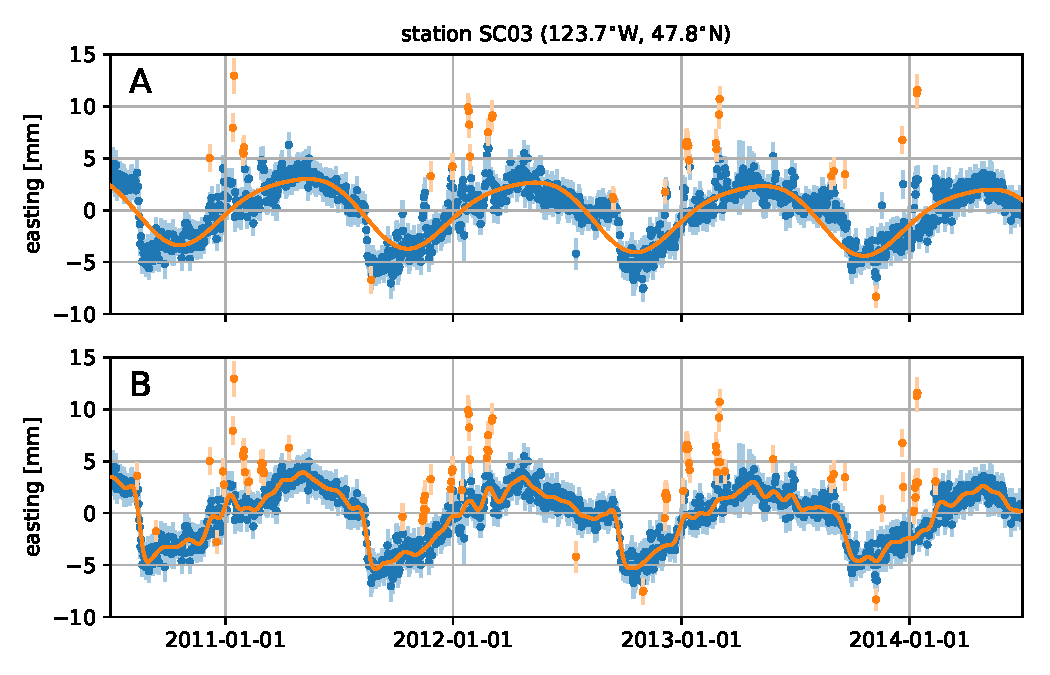
\includegraphics{figures/outliers_new/outliers.pdf}
\caption{
Outliers detected in the easting component of displacements at station
SC03. The orange markers indicate detected outliers. The orange line
is the best fit model to the data, which is used to compute the
residual vector $\mitbf{r}$. The model being fit to the data in Panel
A is $\G\mitbf{m}$, and the model in Panel B is $\G\mitbf{m} +
v(\points)$.
}
\label{fig:Outliers}
\end{figure*}

\bibliographystyle{gji}
\bibliography{mybib}  

\end{document}
